%%%%%%%%%%%%%%%%%%%%%%%%%%%%%%%%%%%%%%%%%%%%%%%%%%%%%%%%%%%%%%%%%%%%%%%%%%%%%%%%
%   Chapter 2
%%%%%%%%%%%%%%%%%%%%%%%%%%%%%%%%%%%%%%%%%%%%%%%%%%%%%%%%%%%%%%%%%%%%%%%%%%%%%%%%
\chapter{Graphical User Interface} \label{chap:gui}

%%%%%%%%%%%%%%
% Introduction
\section{Introduction} \label{sec:guiintro}

%%%% Role of the GUI
Before beginning creation of the GUI, a very high level analysis of its role was performed---it was treated as a `black box' system to define inputs and outputs. Neighboring systems which provide input to the GUI are the GPS receivers and the DAF application, and output from the GUI is sent directly to a display device. In order to robustly communicate with the input systems, a single middleware application (described in Sec. \ref{sec:datadiss}) was designed to eliminate unnecessary or redundant data transfer. The result of this `black box' analysis is the information flow architecture depicted in Fig. \ref{fig:blackboxflow}.

% list the output data: dst, dev magnitude and direction
The fundamental purpose of this graphical tool is to show a driver the path which another vehicle has taken, and how to replicate it. So a series of dicrete position goals must be displayed in some manner or frame of reference that is instantly understandable. When the position of the vehicle attempting to follow this path does not coincide with some part of that path, the driver will need to know how large the discrepancy is and how to correct it. Lastly, when visual following becomes unreliable, the risk of rear-end collision is increased, so a follower will need to know how far away the are from the vehicle in front of them and whether this distance is safe. So the GUI will show a relative path, lateral deviation from that path, and curvilinear separation (distance along the path between leader and follower) with a corresponding safety estimate.
% list the input data: pos, vel, crs, path
The inputs necessary to relay that information were then determined to be, at a minimum, the array of two dimensional path points rotated and translated into the following vehicle's coordinated frame, and velocity state of the following vehicle. Later, as development progressed to the state described in Sec. \ref{sec:finaldes_earth}, other inputs were channelled in to augment a following driver's situational awareness further.

% Black box info flow chart
\begin{figure}[ht] \centering 
    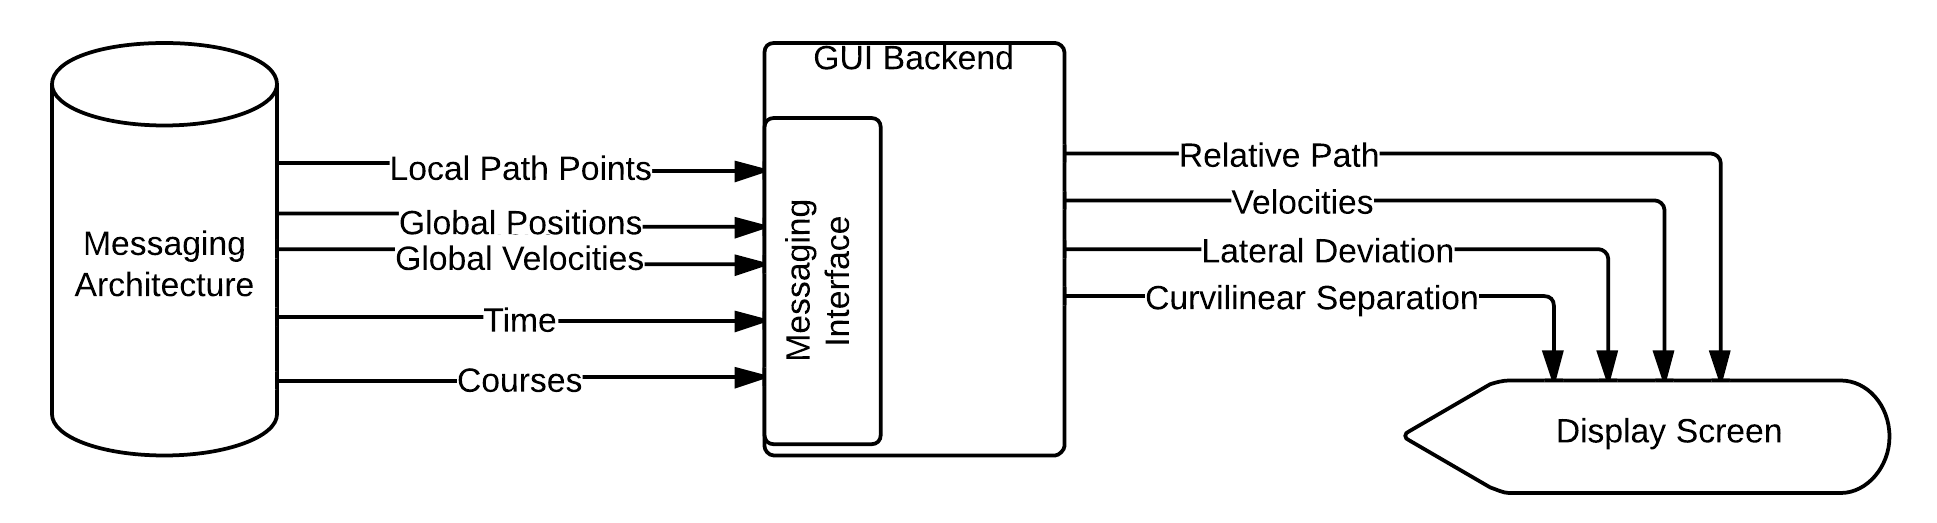
\includegraphics[width=6.5in]{./figs/blackbox_flowchart.png}
    \caption{High level information flow architecture in and out of the GUI} \label{fig:blackboxflow}
\end{figure}

% warn and crit states
When characterizing the statuses of deviation and forward distance, it was determined that a scheme similar to that of U.S. stoplights would be used in order to communicate alerts in a fashion familiar to many drivers; green denotes acceptable conditions, yellow is displayed when warning is merited, and red when a critical boundary has been violated. This coloring is used on the representation of both vehicles to relay two pieces of information: follower color indicates the corresponding value of lateral deviation relative to deviation thresholds, and leader color indicates the corresponding value of forward curvilinear separation distance relative to safe following distance thresholds. The process for determining the exact values for thresholds at which color changes occur is outlined in Sec. \ref{sec:guicalc}.

%%%% Made 2 GUIs
%% Monolith
From the outset, a primary design goal was to minimize the amount of visual and cognitive effort required on the part of the driver for determining whether course and speed corrections are necessary, and if so, what they are. Facilities for accepting driver-input operational parameters must therefore be obscured during the driving task, yet easily accessible on the fly. In addition, a clean and minimal visual presence ensures that a passing glance is sufficient to check on distance and deviations. When following very closely, a follower will need to anticipate upcoming turns without being able to see the leader actually turn, so course information---specifically, the leader's course relative to that of the follower---will be needed.  These were the fundamentals driving the GUI development at the outset. Since the resulting interface was presented in a single window on the display device and utilized only the Qt4 C++ library and associated Python bindings for rendering, it is referred to as `monolithic'.

%% Earth
Since a significant end use case involves military convoys, feedback was sought from personnel in the Armed Forces. One primary criticism was the lack of visual stimuli by which to reconcile the screen output with what the user sees around them. In essence, it was suggested, users must develop a trust with any tool before beginning to make decisions based upon it, particularly in the dire situations for which this tool is designed. To remedy this, it was proposed that satellite imagery be incorporated into the background of the information already displayed on the screen. As this directly contradicted the clean, distraction-free nature of the prototype already developed, it was determined that another version needed to be constructed following these new design principals, and that the two GUI's should be juxtaposed the most prudent approach. In determining what software package to use as an imagery backend, a trade study was performed and the resulting candidates were narrowed to Quantum GIS and Earth (by Google). The maturity, user-base and documentation on representing data with the Keyhole Markup Language (KML) ultimately made Google Earth the favored tool.

%%%%%%%%%%%%%%%%%%%%%%X
% Interpolator Section
\section{Real-Time Interpolation} \label{sec:interp}
%%%%% introductory
The addition of satellite imagery made the user highly aware of the update rate of each piece of information displayed spatially, necessitating the incorporation of data smoothing techniques. Since the end goal is to display information that has been received rather than predict future states, a minimum of two most recent data points is required to do a live interpolation. With this, a continuous-time linear interpolation of the measurement at any instant between those two times is possible. By making more data points available and considering the type or nature of data in question, more accurate form of interpolation may be possible. However, due to speed and efficiency, the linear interpolation is preferable in this situation. All values which are displayed in the GUI (listed in Sec. \ref{sec:guiintro}) are passed through the interpolation algorithm.
%%%%% general algorithm
Equation \eqref{eq:interp} gives general form of the linear interpolation to obtain a value $x$ at time $t$ which lies between values $x_0$ and $x_1$ corresponding to times $t_0$ and $t_1$, respectively.
%% formula
\begin{align} \label{eq:interp}
    x(t) &= (x_1 - x_0) \frac{ t - t_0 } { t_1 - t_0 } + x_0
\end{align}

%%%% data-type specific
For two dimensional positions, this procedure is carried out on both the East and North coordinates. 
%% angle
Angles are a different matter. The course dimension contains an inherent discontinuity due to `wrapping' at the North axis. A course change of $-1^\circ$ may result in a measurement change of $-359^\circ$, which if naively interpolated would result in a complete spin over a full timestep, ending at essentially the same location as the beginning. For this reason, the angles must be occasionally be resolved (i.e., when $|x_1 - x_0| > 180^\circ$ ) by adding $360^\circ$ to the lowest value. For example, values of $(x_0, x_1) = (0.5^\circ, 359.5^\circ)$ would then become $(x_0, x_1) = (360.5^\circ, 359.5^\circ)$ .  This value is then checked and corrected by the display controller upon rendering.
%% path
For the path to be interpolated,  the same procedure for positions is carried out for each point in the vector. A problem arises when interpolating between timesteps with unequal numbers of points, as each point cannot then be interpolated as if it were travelling along a line. When path length mismatch occurs between two successive updates, redundant points are added coincident with the rearmost path point until the two vectors are equal in length. When the number of points is decreasing, this alone would lead to a buildup of unnecessary data points, tying up valuable memory space and processing time. Thus, each time the length decreases and stays constant or continues decreasing for two or more timesteps, redundant points are removed from the saved vector.

%% time update
While GNSS provides the ability to precisely synchronize systems, display smoothing must rely upon computer-specific timestamps as some machines will operate more slowly than others. Accordingly, when initial measurement messages arrive, the CPU time at which the content of each message packet was extracted is stored along with that content. It is important that CPU time is recorded upon extraction rather than upon completion of processing or transmission, as the goal of this process is to obscure lags incurred during calculation or radio transmission; the extraction (and assignment) time represents the earliest point when any portion of the rest of the GUI may then access that data to display it. The end result is that the user is presented with data which will change at a consistent frequency (as specified by the user), regardless of whether multiple sensors take varying amounts of time to relay or calculate data.

Upon each subsequent measurement update, the two previously newest values $(x_1,t_1)$ are moved to variables for old data $(x_0, t_0)$ and the new value is stored along with present CPU time. An interpolation object representing Eq. \eqref{eq:interp} is created with the present data so that between times $t_0$ and $t_1$ an input $t$ will yield the respective measurement $x$. Any interpolation thread which is still running is then stopped, and a new one spawned. This thread begins incrementally calculating data between $x_0$ and $x_1$, then waits a period of time corresponding to the desired frequency, repeating until either a new measurement update occurs or time $t_1$ is reached.

%%%%% transition to data dissemanation
The effect this had upon readability and being able to intuitively interpret data was positive. Even though it was initially intended to smooth movement of satellite imagery and low sensor frequencies, it became desirable to investigate the benefits on the monolithic GUI. Rather than rewrite the smoothing tool for that purpose, it was modularized as described in Sec. \ref{sec:datadiss}, to distribute data agnostically.

%%%%%%%%%%%%%%%%%%%%
% Data Dissemenation
\section{Data Dissemenation} \label{sec:datadiss}

When creating an application to run in realtime, it is of utmost importance that infomation be passed about in a prudent manner, or latency will accumulate and render the application  useless. The MOOS framework \cite{moos} was already in place for communication between the DRTK, TDCP, and DAF algorithms, and the GPS receivers used. However, it is desireable to have a middleware interface that can easily accomodate a data stream incoming from any middleware, and be attached to the GUI in an agnostic manner with minimal effort. Furthermore, in designing the real-time interpolation described in Sec. \ref{sec:interp}, it became apparent that the process needed to be performed at the earliest possible instance to avoid over-complication with the GUI itself. During testing and debugging of the interpolator, an alternative approach was needed to verify its functionality, so a scheme was devised whereby all measurements were held until the slowest measurement---the path vector---had been updated, so integration of this was needed as an option. To summarize, a middleware interface was needed to agnostically and robustly join with any number of messaging frameworks, perform a real-time interpolation on all data before doing that---or simply synchronize if so desired---and then pass that data into the GUI. The solution is outlined below, and depicted graphically in Fig. \ref{fig:midw_diagram}.

\begin{figure}[ht] \centering 
    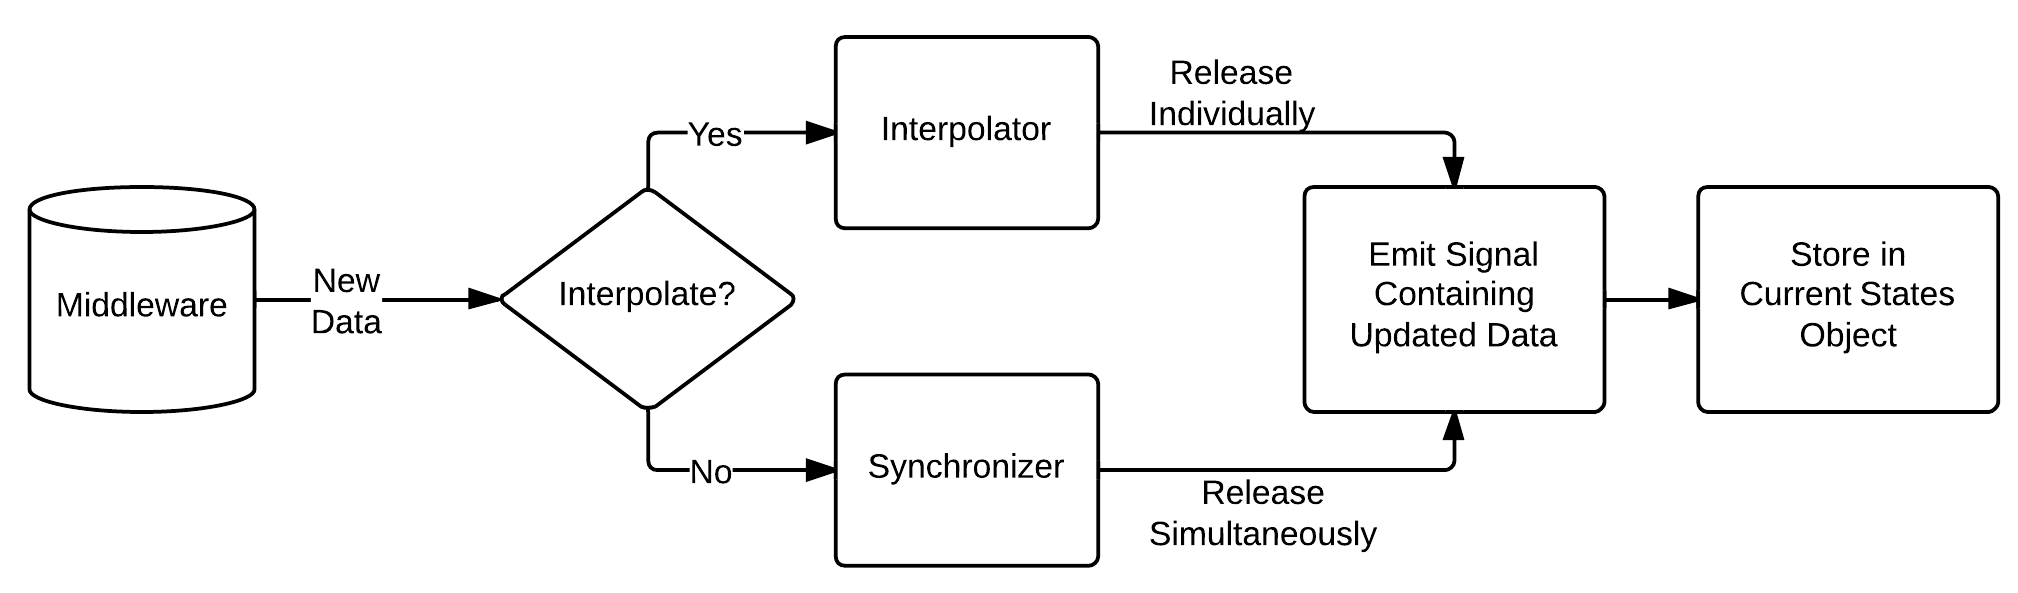
\includegraphics[width=6.5in]{./figs/middleware_diagram.png}
    \caption{Algorithm for interfacing middlewares with the GUI backend} \label{fig:midw_diagram}
\end{figure}

% moos - ok.
MOOS comprises a publisher-subscriber message passing system with a single central database which may hold floating point numbers or strings. The `Messaging Architecture' object in Fig.~\ref{fig:blackboxflow} refers to the MOOS database and its ecosystem, and it serves purely as a source of data, meaning that the `Messaging Interface' object in the same figure is a MOOS application created as a means of retrieving this data and converting it into a useable form.
Both GUIs were initially developed using postprocessed data collected from an Prowler ATV automously following an Infiniti G35---the original use of the DAF algorithm---using the same positioning and radio setup described in Sec. \ref{sec:hardware}. This was made possible by the playback feature of the MOOS framework, which is used to broadcast data from a text file as if it were streaming live.
Sec. \ref{sec:test} describes how selectivity was exercised during data collection to minimize memory usage while maximizing the usefulness of the data that was collected when it was replayed.

%%%% Qt Signals/Slots - alright.
Both GUIs were constructed using the Qt \cite{qt} framework to varying degrees. The interface backend of the monolithic GUI relied entirely upon a Qt window and components, and the command interface of the Earth-based GUI (see Sec. \ref{sec:finaldes_earth}) was constructed similarly. Many items in each window may be changed by the user or update based on incoming data, and must subsequenty interact with other items in the window. For instance, when the user changes a $\mu$ value using the tab in Fig.~\ref{sec:finaldes_monolith}, the corresponding variable being accessed by the function which calculates stopping distance thresholds must then be changed. Qt has an internal message passing scheme similar to a publisher/subscriber model, using instead what are called signals and slots. Continuing the example above, when that $\mu$ value is changed the `spinbox' by which the user changed it then emits a signal which is broadcast out. It is then received by all connected slots. These signal/slot connections are made at runtime, when the object instances to which they belong are created.

%%% midw interface
% Bridging these two ecosystems is necessary, and 
% In this way GUI inputs can be made agnostic to the middleware used, requiring only a simple widget be written in order to be hooked up to a new data stream. 
%%% midw interface was where interpolation was performed

%%%% Specific to Earth GUI - alright.
%% KML server
Every detail displayed in the Earth GUI at any instant is defined using a document written in the Keyhole Markup Language. These documents must be generated at whatever screen refresh rate is desired. Supplying KML documents updating in excess of 10 Hz required contsruction of a local server which was built using the Tornado web framework. Each KML document contains 3D view information supplied by the controls located in a view tab located in the command interface described in Sec. \ref{sec:finaldes_earth}. The object which is controlled is a virtual camera perspective above the satellite imagery specified by a point of focus on which to center the screen (determined by a combination of vehicle positions), altitude above that point, tilt from vertical, and heading relative to north.
%% passing middleware object instance references
All this information is easily accessible in a central location by creating a single information object. A reference to this instance is passed to all applications which need to either update it with new data or retrieve a snapshot of the latest data from it. In this manner, creation of alternative middleware interfaces is greatly simplified.


%%%%%%%%%%%%%%
% Calculations
%%%%%%%%%%%%%%
\section{Calculations} \label{sec:guicalc}

% UTM coordinates - REDO
When displaying data on a rectangular screen, it becomes desirable to utilize a coordinate system more suited to cartesian calculations than Latitude-Longitude-Altitude (LLA), one which employs standard metric units of length. Whenever rectangular coordinates are necessary the Universal Transverse Mercator (UTM) east and north representations of global positions are used. The conversions between the LLA and UTM coordinate systems are outlined in \cite{projections}.

%%%% Calculating the lateral error
The most crucial calculations are performed upon the vector of relative path points, of which two particular points are the subject of great attention. In Fig. \ref{fig:pathpts} the point $(x_1,y_1)$ represents the nearest (i.e., lowest distance to the origin) which also lies behind the antenna of following vehicle, meaning the vector from the origin and the follower's velocity vector form an obtuse angle. The DAF algorithm sorts and outputs points such that this will be the last in the vector, and prior to this will be the nearest point in front of the vehicle's antenna, named $(x_2,y_2)$ in Fig. \ref{fig:pathpts}. The path is assumed to be straight between these two points. The lateral deviation of a follower at $(x_0, y_0)$ from the path occurs here and is defined as the length of a line perpendicular to the path line, which it intersects at $(x_3,y_3)$---used later for forward spacing calculation. Note that depending on path shape and timing, $(x_3,y_3)$ may not necessarily lie between $(x_1,y_1)$ and $(x_2,y_2)$. Since the DAF algorithm will output in East-North coordinates translated to the follower's position, $(x_0, y_0)=(0,0)$ at all times. The formulation of the lateral deviation is then given by Eq. \eqref{eq:laterr} \cite{laterrformula}. 
% Lateral error formula
\begin{align} \label{eq:laterr}
    e &= \frac{ | (x_2 - x_1)(y_1 - y_0) - (x_1 - x_0)(y_2 - y_1) | } { \sqrt{ (x_2 - x_1)^2 + (y_2 - y_1)^2 } }
\end{align}
The underlying assumption here is that the GPS antenna is placed on the lateral center of the vehicle. Once this value has been determined, it may simply be compared against user-input threshold values for warning and critical states to determine whether to issue an alert as discussed in Secs. \ref{sec:finaldes_monolith} and \ref{sec:finaldes_earth}.

% pathpts diagram
\begin{figure}[ht] \centering
\begin{tikzpicture}[
        scale=5,
        axis/.style={thin, ->, >=stealth'},
        every node/.style={circle, color=black}   ]
    % axis
    \draw[axis] (-0.1,0) -- (0.2,0) node(xline)[right] {$X$};
    \draw[axis] (0,-0.1) -- (0,0.2) node(yline)[above] {$Y$};
    % points
    \coordinate (a) at (0.35,0.35);
    \coordinate (b) at (0.6,0.6);
    \coordinate (c) at (0.85,0.85);
    \coordinate (d) at (0.85,0.35);
    % right angle
    \tkzMarkRightAngle[fill=gray!20,size=.05](a,b,d)
    \node[draw,circle,inner sep=2pt,fill=blue] at (a) {};
    \node[draw,circle,inner sep=2pt,fill=green] at (b) {};
    \node[draw,circle,inner sep=2pt,fill=blue] at (c) {};
    \node[draw,circle,inner sep=2pt,fill=red] at (d) {};
    % point labels
    \node [below left] at (a)  {$(x_1,y_1)$};
    \node [left] at (b)  {$(x_3,y_3)$};
    \node [above right] at (c) {$(x_2,y_2)$};
    \node [below right] at (d) {$(x_0,y_0)$};
    % path arrow
    \draw[very thick,blue,->] (a) -- (c) node [pos=0.75, sloped, above, color=blue] {path};
    % dev arrow
    \draw[very thick,red,->] (d) -- (b) node [pos=0.5, sloped, above, color=red] {dev};
\end{tikzpicture}
\caption{Key path points near to the follower} \label{fig:pathpts}
\end{figure}

%%%% Calculating the distance
Next, a measure of the curvilinear distance separating the leader and follower is necessary for collision avoidance purposes. To do this, it is assumed that the follower will adhere to the path, and that the current position of the follower lies along rearmost path line at point $(x_3, y_3)$ where $m_{12}$ and $m_{03}$ represent the slopes of the rearmost path line and the perpendicular deviation line, respectively. Finding this point is possible by use the relations in Eqs. \eqref{eq:devprojx} and \eqref{eq:devprojy}. The line segment between it and $(x_1,y_1)$ is removed, and the magnitudes of all other lines are summed to obtain the curvilinear spacing between the two GPS antennae. 

% projection of deviation point
\begin{align} 
    x_3 &= \frac{ m_{12} x_1 - m_{03} x_0 + y_0 - y_1 } { m_{12} - m_{03} } \label{eq:devprojx} \\
    y_3 &= m_{03} (x_3 - x_0) + y_0 \label{eq:devprojy}
\end{align}

Ultimately, a safety estimate for forward spacing at any given time is to be compared to this distance and used to determine an alert status as described in Secs. \ref{sec:finaldes_monolith} and \ref{sec:finaldes_earth}. For this estimate, a few assumptions are made about the braking behavior: the vehicle in question is equipped with a braking system which is able to keep friction forces between the road and tires in the static regime (anti-lock brakes), the braking system is capable of maintaining peak longitudinal forces during negative acceleration, and the driver has an instantaneous reaction time. At each update, a minimum stopping distance is calculated based on these assumtions for two different road surfaces with user-input coefficients of friction corresponding to the warning and critical states, where $\mu_{crit}<\mu_{warn}$ resulting in $d_{stop, min}^{crit} < d_{stop, min}^{warn}$. This relation is given in Eq. \eqref{eq:stopdist}, where $\mu$  is the combined coefficient of static friction between the terrain surface and the tires,  $|\bar{v}|$ is the magnitude of ground-plane velocity, and $g$ is the acceleration due to gravity.
% stopping distance equation (mu)
\begin{align} \label{eq:stopdist}
    d_{stop, min} &= \left( \frac {1} {\mu g} \right) \left(\frac {|\bar{v}|^2} {2} \right)
\end{align}

The velocity and acceleration terms are separated to emphasize that in this relation, $\mu$ represents a negative acceleration in earth gravities that will be required of the vehicle. The previously stated assumptions are made in order to reduce the number of user-input values for the distance safety calculation to these two alone. The default values are for a low-friction surface such as a dirt or gravel road ($\mu_{crit}=0.5$), and a `critical' state---when the present minimum stopping distance is than that for a typical dry asphalt roadway ($\mu=1.0$) \cite{mu}. 

%%%%%%%%%%%%%%%%%%%%%%
% Final Design Section
\section{Final Design} \label{sec:finaldes}

%%%% Monolith %%%%
\subsection{Monolithic GUI} \label{sec:finaldes_monolith}
The final form of the monolithic GUI can be seen in Figures \ref{fig:finaldesdriv_monolith} and \ref{fig:finaldesopts}. Immediately noticeable is the tabbed `command interface' on the right of the window. It contains two primary tabs: one for display of important data (forward spacing, lateral deviation, and follower velocity), and a tab for entry of operational parameters. The view is always oriented such that `up' on the screen corresponds to the positive longitudinal axis of the following vehicle. The orientation of the lead vehicle (represented with a simple square icon containing an arrow for its positive longitudinal axis) is then always shown relative to the follwing vehicle. So if the leader is shown pointing to the right, the direction of its motion is then parallel to the follower's lateral axis and in the positive direction. A third tab containing controls for manually manipulating the orientation was created, however this was intended only for development purposes and is unavailable to the end user, to prohibit distraction during the driving task. It should be noted as well that all vehicle coordinate frames are in accordance with the Society of Automotive Engineers' Vehicle Axis System \cite{vdbook}.

% the driver screen
\begin{figure}[ht] \centering 
    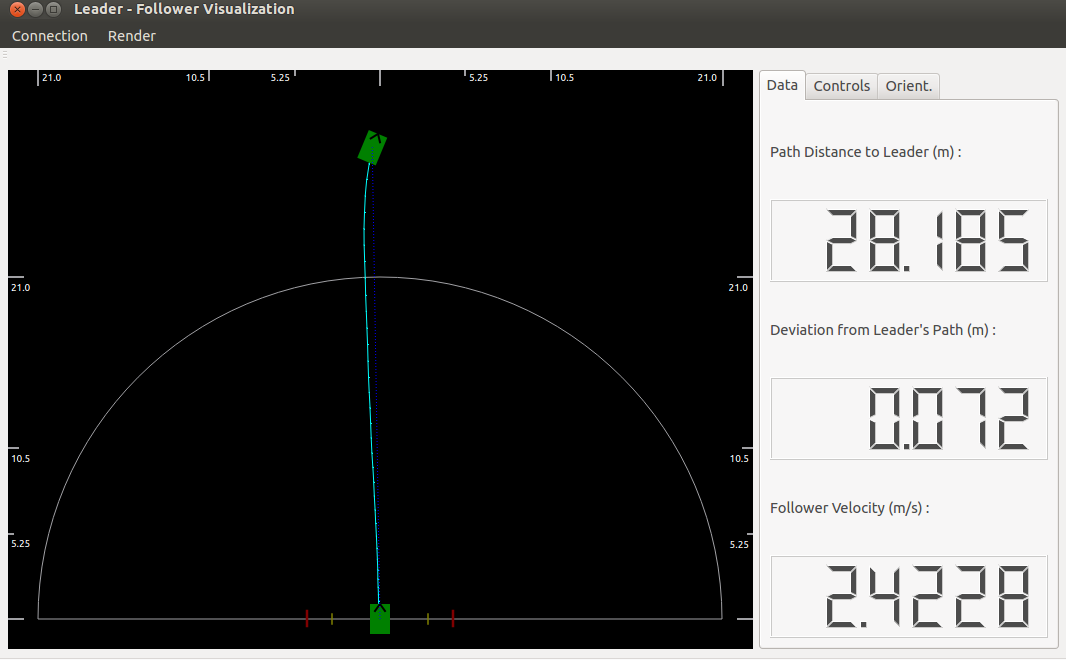
\includegraphics[width=5in]{./figs/final_design_data.png}
    \caption{Final monolithic design --- driver view} \label{fig:finaldesdriv_monolith}
\end{figure}

% the option screen
\begin{figure}[ht] \centering
    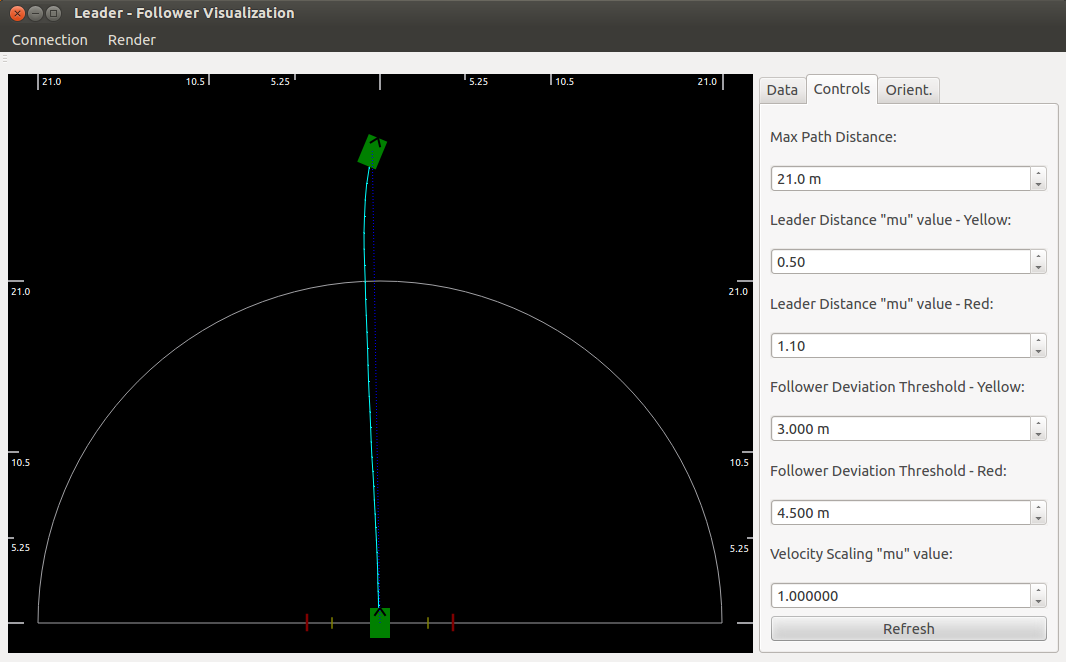
\includegraphics[width=5in]{./figs/final_design_opts.png}
    \caption{Final monolithic design --- setting of operational parameters} \label{fig:finaldesopts}
\end{figure}

%% options screen
A total of five operational parameters may be varied using the screen depicted in Figure \ref{fig:finaldesopts}, four of which are those mentioned in Sec. \ref{sec:guicalc}: the two lateral deviation thresholds and the two following distance $\mu$ thresholds. Since no global coordinates are used here, screen size is directly proportional to east and north distances in meters by some scalar value. To determine this ratio, the user inputs a maximum range distance value corresponding to the outer radius of a range indicator semicircle displayed onscreen. The number of pixels needed to display that semicircle then determines how all other objects are scaled. Since the representions of each vehicle convey important infomation, these features are not allowed to change in size, but rather occupy a constant number of pixels determined by the size of the display device. To assist in communicating the relative lengths represented, scaling legends are placed on the left, right, and top of the black render area where graphics are displayed. The drawback to this constant maximum range display is that the leader may lie outside of it, potentially disorientating the user. However, was curtailed by adding optional functionality for automatically scaling the view screen such that the leader is always within the range semicircle. When the option to always display the lead vehicle is enabled, the user-input maximum range distance becomes the minimum value, and whenever the direct distance to the follower exceeds this, the screen is scaled to include it in the range semicircle. The tradeoff is that distances must be determined by reading the values on the legend.

%%%% Earth %%%%
\subsection{Google Earth GUI} \label{sec:finaldes_earth}

With the Earth-based incarnation, design goals had been changed considerably. Since the presence of satellite imagery drastically increases the amount of  visual stimuli, it was decided that the user should be able to enter view-only mode and be rid of any objects designed for input once operational parameters had been settled upon. To this end, the command interface was liberated from the central display screen and forms its own window outside the Earth environment. The command interface backend remains as the object carrying out all mathematical calculations. This makes it simpler to get the current values of any operational parameters needed wihout incurring additional overhead since their values are also attributes of the same object. One valuable feature addition was the ability to focus the satellite camera directly above either vehicle and track its motion. Should one wish to track both, functionality is in place to track the point in space halfway between each. Should they move too far apart to view, zoom controls allow refocusing the image.

%%%% alerts - TODO get a shot with the data screen
\begin{figure}[ht] \centering 
    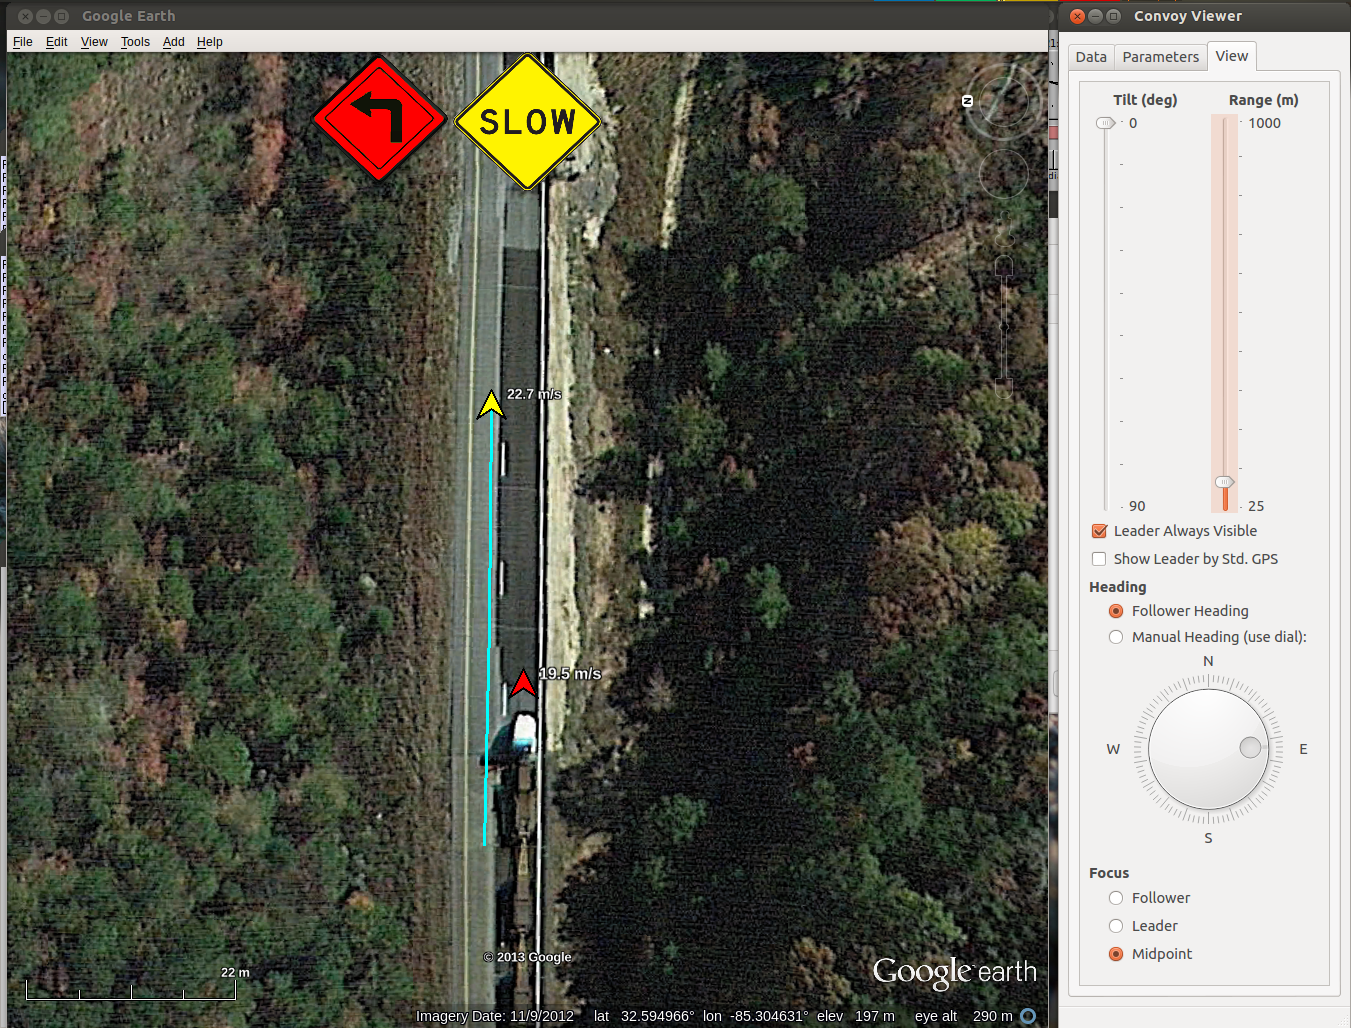
\includegraphics[width=5in]{./figs/earth_slow.png}
    \caption{Following driver being signalled in Google Earth to correct left and slow} \label{fig:earth_dst}
\end{figure}

Figure \ref{fig:earth_dst} depicts both leader and follower on a straightaway, with the follower travelling too fast and too closely to the leader for acceptable safety limits, but within critical boundaries. As such, a yellow traffic sign depiction is presented to the driver communicating the need to reduce speed, thus increasing the separation distance. Being all the way in the wrong lane to the right of the path, the lateral deviation has passed out into a critical state, so a red traffic sign depiction is displayed which communicates to the driver the need to correct left.

% TODO Range/tilt/heading information
